\documentclass[12pt,letterpaper]{article}
\usepackage{graphicx,textcomp}
\usepackage{natbib}
\usepackage{setspace}
\usepackage{fullpage}
\usepackage{color}
\usepackage[reqno]{amsmath}
\usepackage{amsthm}
\usepackage{fancyvrb}
\usepackage{amssymb,enumerate}
\usepackage[all]{xy}
\usepackage{endnotes}
\usepackage{lscape}
\newtheorem{com}{Comment}
\usepackage{float}
\usepackage{hyperref}
\newtheorem{lem} {Lemma}
\newtheorem{prop}{Proposition}
\newtheorem{thm}{Theorem}
\newtheorem{defn}{Definition}
\newtheorem{cor}{Corollary}
\newtheorem{obs}{Observation}
\usepackage[compact]{titlesec}
\usepackage{dcolumn}
\usepackage{tikz}
\usetikzlibrary{arrows}
\usepackage{multirow}
\usepackage{xcolor}
\newcolumntype{.}{D{.}{.}{-1}}
\newcolumntype{d}[1]{D{.}{.}{#1}}
\definecolor{light-gray}{gray}{0.65}
\usepackage{url}
\usepackage{listings}
\usepackage{color}

\definecolor{codegreen}{rgb}{0,0.6,0}
\definecolor{codegray}{rgb}{0.5,0.5,0.5}
\definecolor{codepurple}{rgb}{0.58,0,0.82}
\definecolor{backcolour}{rgb}{0.95,0.95,0.92}

\lstdefinestyle{mystyle}{
	backgroundcolor=\color{backcolour},   
	commentstyle=\color{codegreen},
	keywordstyle=\color{magenta},
	numberstyle=\tiny\color{codegray},
	stringstyle=\color{codepurple},
	basicstyle=\footnotesize,
	breakatwhitespace=false,         
	breaklines=true,                 
	captionpos=b,                    
	keepspaces=true,                 
	numbers=left,                    
	numbersep=5pt,                  
	showspaces=false,                
	showstringspaces=false,
	showtabs=false,                  
	tabsize=2
}
\lstset{style=mystyle}
\newcommand{\Sref}[1]{Section~\ref{#1}}
\newtheorem{hyp}{Hypothesis}

\title{Problem Set 3}
\date{Due: November 11, 2024}
\author{Applied Stats/Quant Methods 1}


\begin{document}
	\maketitle
	\section*{Instructions}
	\begin{itemize}
		\item Please show your work! You may lose points by simply writing in the answer. If the problem requires you to execute commands in \texttt{R}, please include the code you used to get your answers. Please also include the \texttt{.R} file that contains your code. If you are not sure if work needs to be shown for a particular problem, please ask.
	\item Your homework should be submitted electronically on GitHub.
	\item This problem set is due before 23:59 on Sunday November 11, 2024. No late assignments will be accepted.

	\end{itemize}

		\vspace{.25cm}
	
\noindent In this problem set, you will run several regressions and create an add variable plot (see the lecture slides) in \texttt{R} using the \texttt{incumbents\_subset.csv} dataset. Include all of your code.

	\vspace{.5cm}
		\lstinputlisting[language=R, firstline= 5 , lastline=6] {PS03_answersAR.R}
\section*{Question 1}
\vspace{.25cm}
\noindent We are interested in knowing how the difference in campaign spending between incumbent and challenger affects the incumbent's vote share. 
\begin{enumerate}
		\item Run a regression where the outcome variable is \texttt{voteshare} and the explanatory variable is \texttt{difflog}.
		\lstinputlisting[language=R, firstline= 10 , lastline=12] {PS03_answersAR.R}
		\begin{figure}[h!]\centering
			\caption{\footnotesize Regression between voteshare and difflog}
			\label{}
			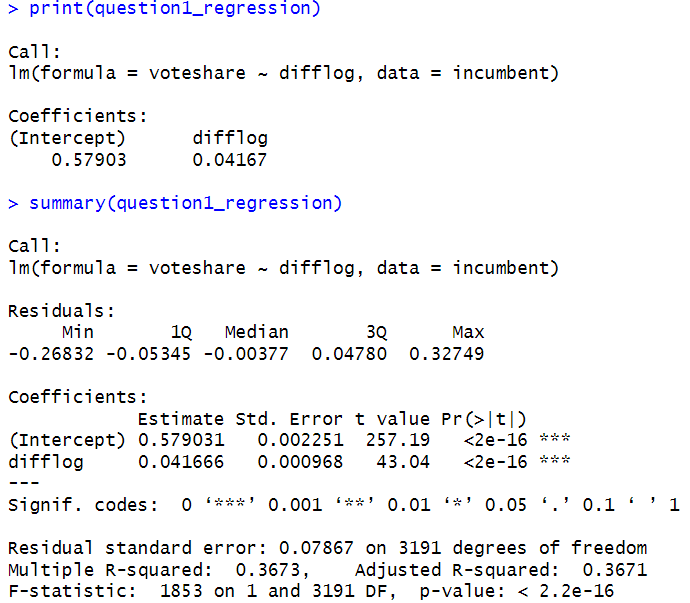
\includegraphics[width=.85\textwidth]{question1_regression.png}
		\end{figure}
			Findings: Based on the model, for every one-unit increase in difflog there is an expected increase of about 0.04 in voteshare. This shows a positive relationship, as difflog increases, voteshare will generally increase as well.
		\vspace{5cm}
		\item Make a scatterplot of the two variables and add the regression line.
		\lstinputlisting[language=R, firstline= 17 , lastline=21] {PS03_answersAR.R}
		\begin{figure}[h!]\centering
			\caption{\footnotesize Question1 Scatter Plot}
			\label{}
			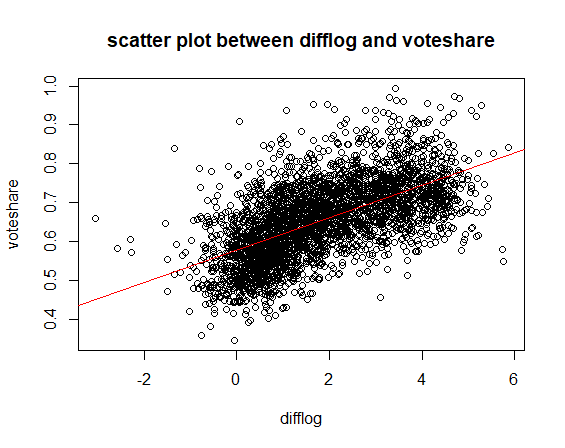
\includegraphics[width=.85\textwidth]{question1_scatter.png} 
		\end{figure}
		\vspace{7cm}
		\item Save the residuals of the model in a separate object.
		\lstinputlisting[language=R, firstline= 24 , lastline=24] {PS03_answersAR.R}
		\item Write the prediction equation.
		\begin{align*}
		\hat{y} &= \hat{\beta_0} + \hat{\beta_1} \times  \text{difflog}\\
		voteshare &= 0.579 + 0.042 \times \text{difflog}
		\end{align*}
		\lstinputlisting[language=R, firstline= 26, lastline=28] {PS03_answersAR.R}
	\end{enumerate}
	
\newpage

\section*{Question 2}
\noindent We are interested in knowing how the difference between incumbent and challenger's spending and the vote share of the presidential candidate of the incumbent's party are related.	\vspace{.25cm}
	\begin{enumerate}
		\item Run a regression where the outcome variable is \texttt{presvote} and the explanatory variable is \texttt{difflog}.	
		\lstinputlisting[language=R, firstline= 32 , lastline=34] {PS03_answersAR.R}
		\begin{figure}[h!]\centering
			\caption{\footnotesize Regression between presvote and difflog}
			\label{}
			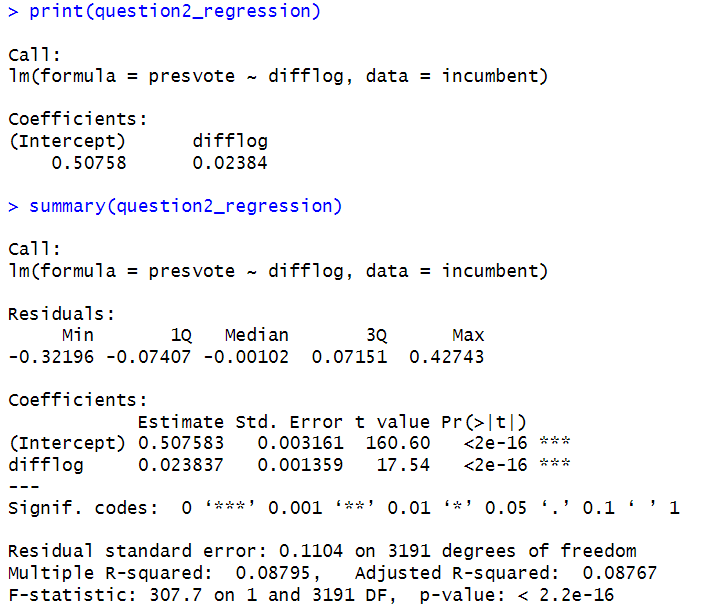
\includegraphics[width=.85\textwidth]{question2_regression.png}
		\end{figure}
		Findings: Based on the model, a one-unit increase in difflog will generally see a 0.02 increase in presvote. This is a positive relationship that shows when difflog rises presvote values tend to slightly increase.
		\vspace{5cm}
		\item Make a scatterplot of the two variables and add the regression line. 	
		\lstinputlisting[language=R, firstline= 39 , lastline=43] {PS03_answersAR.R}
		\begin{figure}[h!]\centering
			\caption{\footnotesize Question 2 Scatter Plot}
			\label{}
			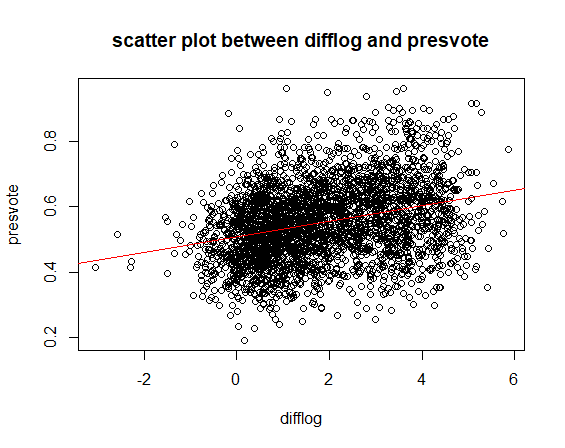
\includegraphics[width=.85\textwidth]{question2_scatter.png} 
		\end{figure}
		\item Save the residuals of the model in a separate object.
		\lstinputlisting[language=R, firstline= 46 , lastline= 46] {PS03_answersAR.R}
		\item Write the prediction equation.
			\begin{align*}
			\hat{y} &= \hat{\beta_0} + \hat{\beta_1} \times  \text{difflog}\\
			presvote &= 0.508 + 0.024 \times \text{difflog}
		\end{align*}
		\lstinputlisting[language=R, firstline= 48, lastline=50] {PS03_answersAR.R}
	\end{enumerate}
	
	\newpage	
\section*{Question 3}

\noindent We are interested in knowing how the vote share of the presidential candidate of the incumbent's party is associated with the incumbent's electoral success.
	\vspace{.25cm}
	\begin{enumerate}
		\item Run a regression where the outcome variable is \texttt{voteshare} and the explanatory variable is \texttt{presvote}.
		\lstinputlisting[language=R, firstline= 54 , lastline= 56] {PS03_answersAR.R}
		\begin{figure}[h!]\centering
			\caption{\footnotesize Regression between presvote and voteshare}
			\label{}
			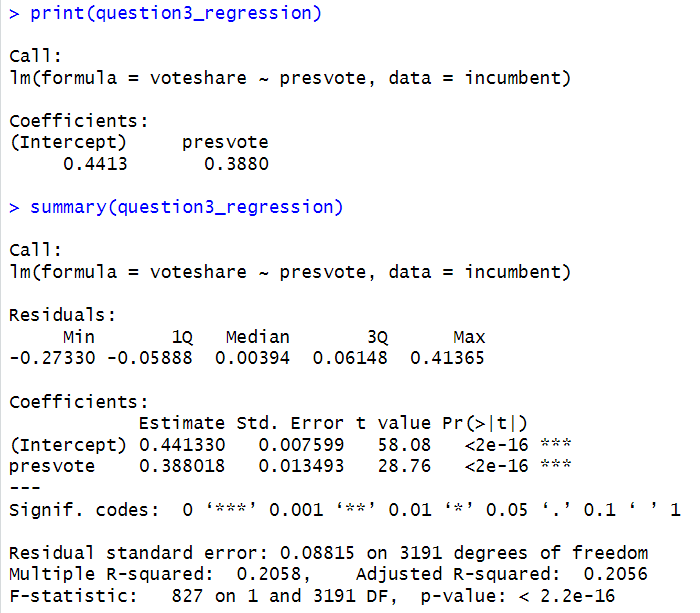
\includegraphics[width=.85\textwidth]{question3_regression.png}
		\end{figure}
		Findings: A one-unit increase in presvote is associated with a 0.38 increase in voteshare. This is a positive relation showing as presvote increases so does voteshare.
			\vspace{5cm}
		\item Make a scatterplot of the two variables and add the regression line. 
		\lstinputlisting[language=R, firstline= 61, lastline= 65] {PS03_answersAR.R}
		\begin{figure}[h!]\centering
			\caption{\footnotesize Question 3 Scatter Plot}
			\label{}
			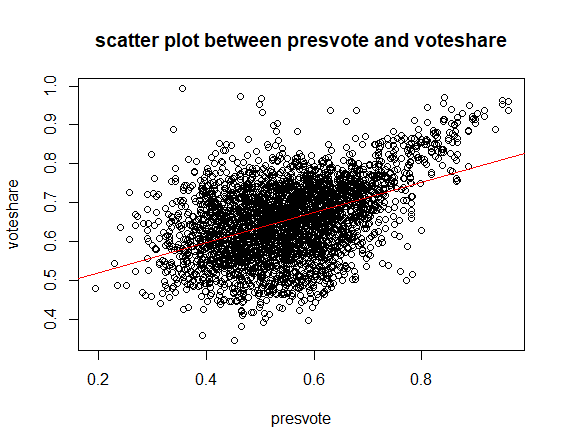
\includegraphics[width=.85\textwidth]{question3_scatter.png} 
		\end{figure}
		\item Write the prediction equation.
		\begin{align*}
			\hat{y} &= \hat{\beta_0} + \hat{\beta_1} \times  \text{presvote}\\
			voteshare &= 0.441 + 0.388 \times \text{presvote}
		\end{align*}
		\lstinputlisting[language=R, firstline= 70, lastline= 72] {PS03_answersAR.R}
	\end{enumerate}
	

\newpage	
\section*{Question 4}
\noindent The residuals from part (a) tell us how much of the variation in \texttt{voteshare} is $not$ explained by the difference in spending between incumbent and challenger. The residuals in part (b) tell us how much of the variation in \texttt{presvote} is $not$ explained by the difference in spending between incumbent and challenger in the district.
	\begin{enumerate}
		\item Run a regression where the outcome variable is the residuals from Question 1 and the explanatory variable is the residuals from Question 2.	
		\lstinputlisting[language=R, firstline= 76 , lastline= 78] {PS03_answersAR.R}
		\begin{figure}[h!]\centering
			\caption{\footnotesize Regression between Q1 residuals and Q2 residuals}
			\label{}
			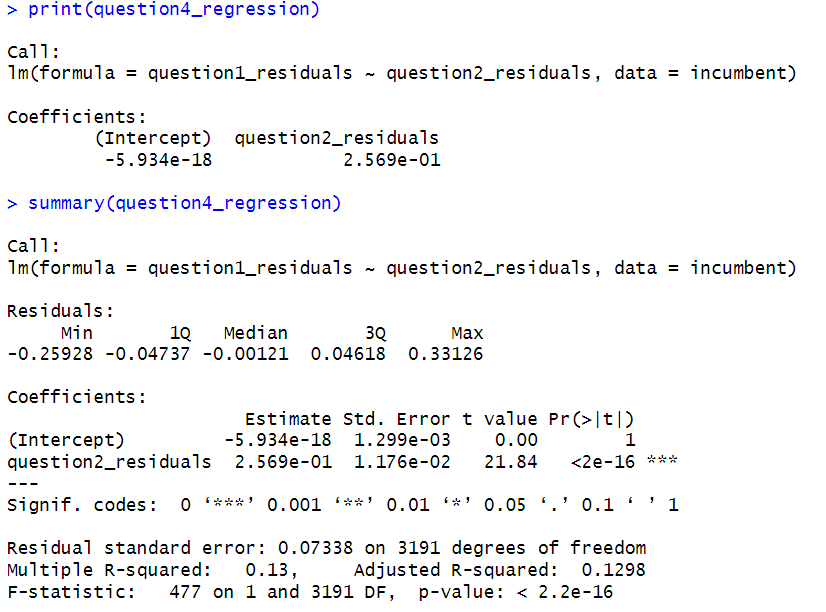
\includegraphics[width=.85\textwidth]{question4_regression.png}
		\end{figure}
			Findings: Running this regression shows if the unexplained parts of presvote (residuals from question 2) help in explaining the remaining variation in voteshare. The positive coefficient of 0.2569 shows that some of the residual variation in presvote can help in explaining the residual variation in voteshare.
		\item Make a scatterplot of the two residuals and add the regression line. 	
		\lstinputlisting[language=R, firstline= 83, lastline= 87] {PS03_answersAR.R}
		\begin{figure}[h!]\centering
			\caption{\footnotesize Question 4 Scatter Plot}
			\label{}
			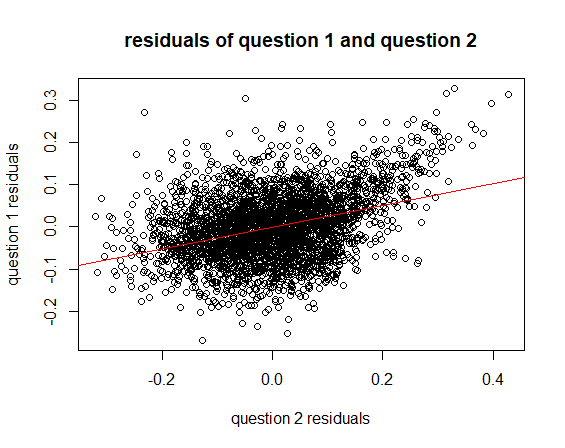
\includegraphics[width=.85\textwidth]{question4_scatter.png} 
		\end{figure}
		\item Write the prediction equation.
		\begin{align*}
			\hat{y} &= \hat{\beta_0} + \hat{\beta_1} \times  \text{question2 residuals}\\
			question1 residuals &= 0 + 0.257 \times \text{question2 residuals}
		\end{align*}
		\lstinputlisting[language=R, firstline= 90, lastline= 92] {PS03_answersAR.R}
	\end{enumerate}
	\newpage	

\section*{Question 5}
\noindent What if the incumbent's vote share is affected by both the president's popularity and the difference in spending between incumbent and challenger? 
	\begin{enumerate}
		\item Run a regression where the outcome variable is the incumbent's \texttt{voteshare} and the explanatory variables are \texttt{difflog} and \texttt{presvote}.	
		\lstinputlisting[language=R, firstline= 96, lastline= 98] {PS03_answersAR.R}
		\begin{figure}[h!]\centering
			\caption{\footnotesize Regression between presvote and difflog}
			\label{}
			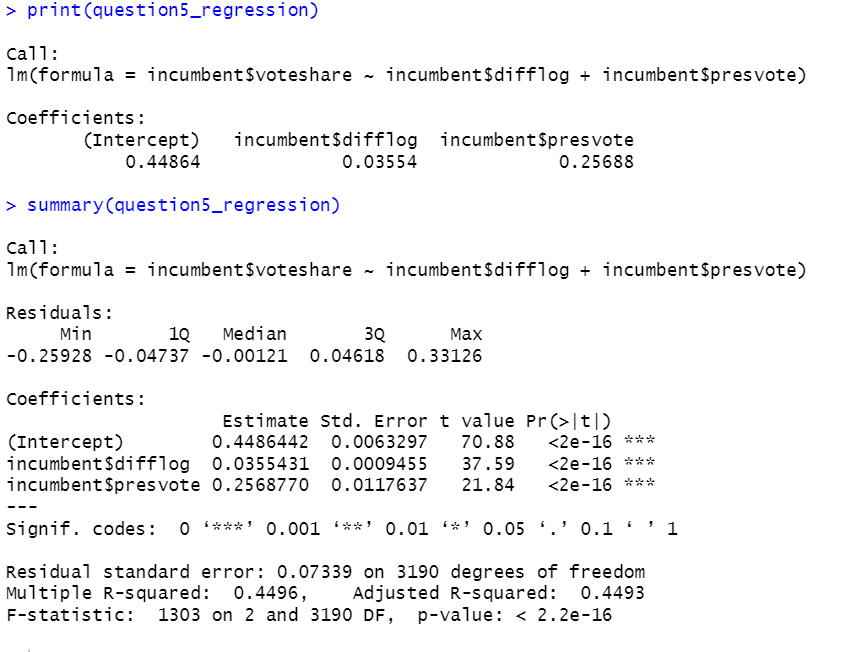
\includegraphics[width=.85\textwidth]{question5_regression.png}
		\end{figure}
		Findings: When presvote is held constant, a one-unit increase in difflog results in a 0.04 increase in voteshare. When difflog is held constant, a one-unit increase in presvote results in a 0.26 increase in voteshare. Both presvote and difflog have positive relationships with voteshare, however, presvote has a stronger impact.
		\item Write the prediction equation.
		\begin{align*}
			\hat{y} &= \hat{\beta_0} + \hat{\beta_1} \times  \text{difflog} + \hat{\beta_2} \times \text{presvote}\\
			voteshare &= 0.449 + 0.036 \times \text{difflog} + 0.257 \times \text{presvote}
		\end{align*}
		\lstinputlisting[language=R, firstline= 48, lastline=50] {PS03_answersAR.R}
		
		\item What is it in this output that is identical to the output in Question 4? Why do you think this is the case?
	
		The coefficient for presvote in Question 5 is identical to Question 4's coefficient for the residual of Question2 (0.257). This shows that after accounting for difflog, in question 5, there is still a partial, additional effect of presvote on voteshare. The 0.257 is a representation of the independent relationship between presvote and voteshare after removing the influence of difflog.
	\end{enumerate}




\end{document}
